\documentclass{boi2014-de}

\usepackage{enumitem}

\renewcommand{\DayNum}{2}
\renewcommand{\TaskCode}{portals}
\renewcommand{\TaskName}{Portals}
\renewcommand{\TaskVersion}{1.1}

\newcommand{\constant}[1]{{\tt #1}}

\begin{document}
    \begin{wrapfigure}[4]{r}{4cm}
        \vspace{-24pt}
		\includegraphics[width=4cm]{\TaskCode.jpeg}
	\end{wrapfigure}
	
    Ein Kuchen, den du unbedingt verspeichen willst, wurde in einem Labyrinth versteckt. Du hast eine Karte des Labyrinths in Form eines Rasters mit $R$ Reihen und $C$ Spalten. Jede Zelle enthält eines der Folgenden Zeichen:
    \begin{description}[itemindent=1pt]
    	\item[\constant{\#}] ist eine Wand,
        \item[\constant{.}] ist ein freies Feld,
        \item[\constant{S}] ist das freies Feld, auf dem du startest,
        \item[\constant{C}] ist das freies Feld mit dem Kuchen.
    \end{description}
    
    Du kannst nur von einem freien Feld zu einem anderen gehen, wenn sie eine gemeinsame Seite haben. Außerdem ist das gesamte Gebiet von einer Wand umgeben ohne jedwedes freie Feld.
    
    Um möglichst schnell an den Kuchen zu kommen, hast du dir ein mobiles Portalgerät von Aperture Science\texttrademark{} besorgt, das wie folgt funktioniert.
    Du kannst jederzeit ein Portal in eine der Vier Kardinalrichtungen (open, unten, rechts, links) schießen. Wenn du ein Portal schießt fliegt es geradeaus, bis es an eine Wand gelangt, an der dann ein Portal erzeugt wird (das Portal ist also dir zugewandt).
    
    Zu jedem Zeitpunkt können höchstens zwei Portal gleichzeitig existieren. Falls bereits zwei vorhanden sind, während du ein neues erzeugst, so verschwindet eines der alten Portale deiner Wahl. Beachte das sich zwei Portale auf verschiedenen Seiten der gleichen Wand befinden können, aber nicht auf der gleichen (das würd ja auch keinen Sinn machen).
    
    Sobald zwei Portale platziert sind, kannst du dich nach belieben zwischen diesen hin und her bewegen. Das heißt wenn du dich auf dem offenen Feld neben einem Portal befindest, kannst du dich auf das offene Feld neben dem anderen Portal bewegen. %Dafür brauchst du genausoviel Zeit, wie du benötigst um ohne Portal auf ein benachbartes Feld zu gehen.
    
    Das erzeugen der Portale benötigt keine Zeit, und die Teleportation durch Portale sowie die normale Bewegung auf ein benachbartes Feld benötigen einen Zeitschritt.

    \Task
    Gegeben die Karte mit Startposition und Position des Kuchens, berechne die minimale Zeit die du benötigst, um den Kuchen zu erreichen.

    \Input
    Die erste Zeile der Eingabe enthält zwei ganze Zahlen, die Anzahl der Zeilen $R$ und die Anzahl der Spalten $C$.
    Die nächsten $R$ Zeilen beschreiben das Labyrinth. Jede dieser Zeilen enthält $C$ Zeichen: \constant{\#},
    \constant{.}, \constant{S} or \constant{C} (deren Bedeutung oben erklärt wurde).
    Dabei tauchen die Zeichen \constant{S} und \constant{S} jeweils genau einmal auf.
    
    Du kannst davon ausgehen, dass es möglich ist den Kuchen von der Startposition aus zu erreichen.

    \Output
    Die Ausgabe soll eine einzige ganze Zahl enthalten --- die minimale Zeit, die du benötigst, um den Kuchen zu erreichen.

    \Example
    \example
    {
        4 4\newline
        .\#.C\newline
        .\#.\#\newline
        ....\newline
        S...
    }
    {
        4
    }
    {
        Ein schnellste Folge von Zügen ist die Folgende: 1) Schritt nach rechts, 2) schritt nach rechts, Portal nach oben und Portal nach unten schießen, 3) bewege dich durch das untere Portal, 4) Schritt nach rechts und nom-nom-nom den Kuchen.

        \begin{center}
            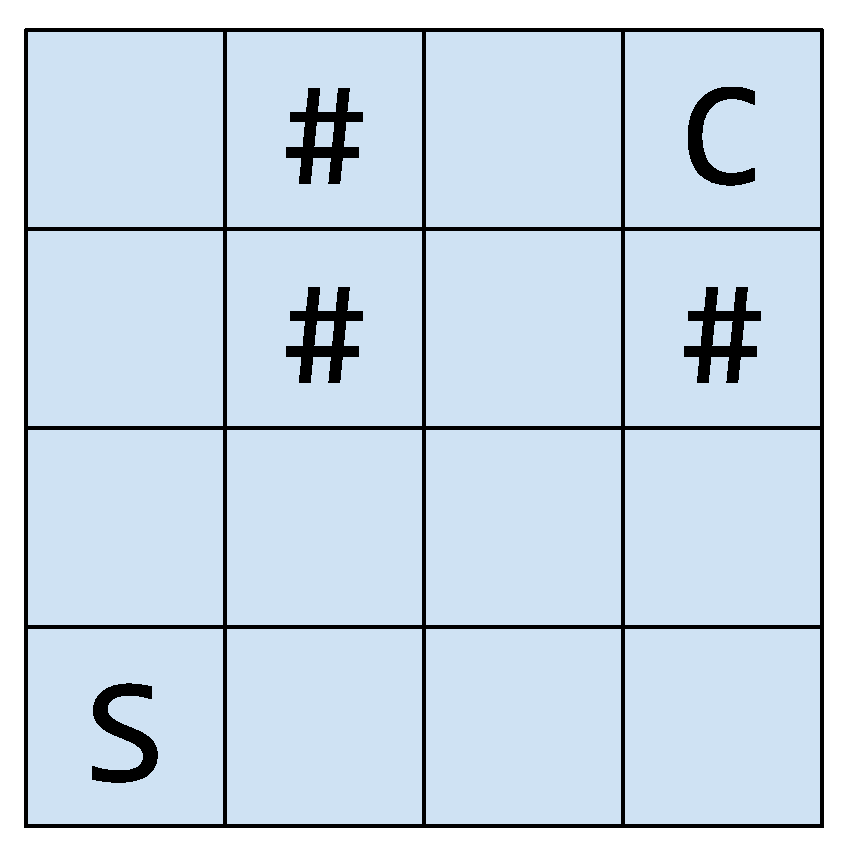
\includegraphics[width=4cm]{portals-example}
        \end{center}
    }

    \Scoring

    \begin{description}[leftmargin=0pt]
        \item[Teilaufgabe 1 (11 points):] $0 \le R \le 10, 0 \le C \le 10$.
        \item[Teilaufgabe 2 (20 points):] $0 \le R \le 50, 0 \le C \le 50$.
        \item[Teilaufgabe 3 (20 points):] $0 \le R \le 200, 0 \le C \le 200$.
        Jedes freie Feld grenzt direkt an mindestens eine Wand.
        \item[Teilaufgabe 4 (19 points):] $0 \le R \le 200, 0 \le C \le 200$.
        \item[Teilaufgabe 5 (30 points):] $0 \le R \le 1000, 0 \le C \le 1000$.
    \end{description}

    \Constraints

    \begin{description}
        \item[Zeitlimit:] ? s.
        \item[Speicherlimit:] ? MB.
    \end{description}
\end{document}
